\PassOptionsToPackage{table,svgnames,dvipsnames}{xcolor}
\documentclass[11pt,a4paper]{article}

% ---------- packages ----------
\usepackage[utf8]{inputenc}
\usepackage[T1]{fontenc}
\usepackage{lmodern}
\usepackage[margin=2.3cm]{geometry}
\usepackage{amsmath,amssymb,amsthm}
\usepackage{xcolor}
\usepackage[most]{tcolorbox}
\usepackage{graphicx}
\usepackage{booktabs}
\usepackage{colortbl}
\usepackage{array}
\usepackage{enumitem}
\usepackage{microtype}
\usepackage{caption}
\usepackage{listings}
\usepackage{fancyhdr}
\usepackage{titlesec}
\usepackage[colorlinks=true,linkcolor=cblue,urlcolor=cteal,citecolor=cgrape]{hyperref}

% ---------- colours ----------
\definecolor{cblue}{HTML}{3B5BDB}
\definecolor{cteal}{HTML}{0CA678}
\definecolor{camber}{HTML}{E8890C}
\definecolor{cred}{HTML}{E03131}
\definecolor{cgray}{HTML}{495057}
\definecolor{cgrape}{HTML}{9C36B5}
\definecolor{ccyan}{HTML}{1098AD}
\definecolor{cpink}{HTML}{E64980}
\definecolor{cink}{HTML}{212529}
\definecolor{codebg}{HTML}{FBF7EE}
\definecolor{rowtint}{HTML}{EEF2FF}

% ---------- section styling (coloured, with rules) ----------
\titleformat{\section}[hang]
  {\color{cblue}\Large\bfseries}{\color{camber}\thesection}{0.6em}{}[{\color{cblue!30}\titlerule[1.1pt]}]
\titleformat{\subsection}
  {\color{cink}\large\bfseries}{\color{cteal}\thesubsection}{0.6em}{}
\titleformat{\subsubsection}
  {\color{cgray}\normalsize\bfseries}{\color{cgrape}\thesubsubsection}{0.6em}{}

% ---------- running header/footer ----------
\pagestyle{fancy}
\fancyhf{}
\renewcommand{\headrulewidth}{0.8pt}
\renewcommand{\headrule}{\hbox to\headwidth{\color{cblue!40}\leaders\hrule height \headrulewidth\hfill}}
\fancyhead[L]{\small\color{cblue}\bfseries Third-Generation Panel Econometrics}
\fancyhead[R]{\small\color{cgray}\leftmark}
\fancyfoot[L]{\small\color{cgray} Dr Merwan Roudane}
\fancyfoot[R]{\small\color{cgray}\thepage}
\renewcommand{\sectionmark}[1]{\markboth{#1}{}}

% ---------- callout boxes ----------
\newtcolorbox{definition}[1][Definition]{breakable,colback=cblue!6,colframe=cblue,
  coltitle=white,fonttitle=\bfseries\small,title={#1},boxrule=0.8pt,arc=3pt,
  left=6pt,right=6pt,top=4pt,bottom=4pt}
\newtcolorbox{keyidea}[1][Key idea]{breakable,colback=camber!8,colframe=camber,
  coltitle=white,fonttitle=\bfseries\small,title={#1},boxrule=0.8pt,arc=3pt,
  left=6pt,right=6pt,top=4pt,bottom=4pt}
\newtcolorbox{begbox}[1][For beginners]{breakable,colback=cteal!7,colframe=cteal,
  coltitle=white,fonttitle=\bfseries\small,title={#1},boxrule=0.8pt,arc=3pt,
  left=6pt,right=6pt,top=4pt,bottom=4pt}
\newtcolorbox{warnbox}[1][Watch out]{breakable,colback=cred!6,colframe=cred,
  coltitle=white,fonttitle=\bfseries\small,title={#1},boxrule=0.8pt,arc=3pt,
  left=6pt,right=6pt,top=4pt,bottom=4pt}
\newtcolorbox{exbox}[1][Worked example]{breakable,colback=cgrape!6,colframe=cgrape,
  coltitle=white,fonttitle=\bfseries\small,title={#1},boxrule=0.8pt,arc=3pt,
  left=6pt,right=6pt,top=4pt,bottom=4pt}
% highlighted equation box
\newtcolorbox{eqbox}[1][]{colback=ccyan!6,colframe=ccyan,boxrule=0.8pt,arc=3pt,
  left=6pt,right=6pt,top=3pt,bottom=3pt,title={#1},coltitle=white,fonttitle=\bfseries\small}

% ---------- Stata code listings (coloured) ----------
\lstdefinelanguage{StataL}{
  morekeywords={xtset,webuse,summarize,describe,use,regress,xtreg,generate,replace,
    xtpkpss,xtpqroot,xtlmbreak,xtpcointegwe,xtpcointegboot,xtbreakcoint,xtccecoint,
    xtcadfcoint,xtnonlincoint,xtbreakmodel,xtcbc,xtkpybreak,xtbfkbreak,xtquantilebreak,
    xtdynestimb,xtpvarcoint,xtgets,xtcd2,xtcsd,test,estimates,matrix,display},
  sensitive=true, morecomment=[l]{*}, morecomment=[l]{//}, morestring=[b]",
}
\lstset{
  language=StataL, basicstyle=\ttfamily\footnotesize\color{cink},
  backgroundcolor=\color{codebg}, keywordstyle=\color{cblue}\bfseries,
  commentstyle=\color{cteal}\itshape, stringstyle=\color{camber},
  frame=single, framesep=5pt, rulecolor=\color{cgray!35}, xleftmargin=6pt,
  breaklines=true, showstringspaces=false, columns=fullflexible, aboveskip=6pt, belowskip=6pt,
}

% ---------- shortcuts ----------
\newcommand{\R}{\mathbb{R}}
\newcommand{\E}{\mathbb{E}}
\newcommand{\Ito}{I(1)}
\newcommand{\Izero}{I(0)}
\newcommand{\cmd}[1]{\texttt{\textcolor{camber}{#1}}}
\newcommand{\hlt}[2]{\textcolor{#1}{\textbf{#2}}}
\newcommand{\bbeta}{\boldsymbol{\beta}}
\newcommand{\bgamma}{\boldsymbol{\gamma}}
\newcommand{\bx}{\mathbf{x}}
\newcommand{\bff}{\mathbf{f}}
\newcommand{\btheta}{\boldsymbol{\theta}}
\newcommand{\bdelta}{\boldsymbol{\delta}}
\newcommand{\bphi}{\boldsymbol{\phi}}
\newcommand{\bpsi}{\boldsymbol{\psi}}
\newcommand{\bxi}{\boldsymbol{\xi}}
\newcommand{\blambda}{\boldsymbol{\lambda}}
\newcommand{\balpha}{\boldsymbol{\alpha}}

\theoremstyle{definition}
\newtheorem{step}{Step}

\begin{document}

% ======================= TITLE =======================
\begin{titlepage}
\thispagestyle{empty}
\centering
\vspace*{0.6cm}
{\color{cblue}\Huge\bfseries Third-Generation Panel Data\\[4pt] Econometrics\par}
\vspace{0.4cm}
{\color{camber}\rule{0.5\linewidth}{2pt}}\par
\vspace{0.4cm}
{\color{cink}\LARGE Structural Breaks and Cross-Sectional Dependence\par}
\vspace{0.35cm}
{\color{cteal}\large A Complete Lecture from Zero --- for Beginners\par}
\vspace{0.9cm}
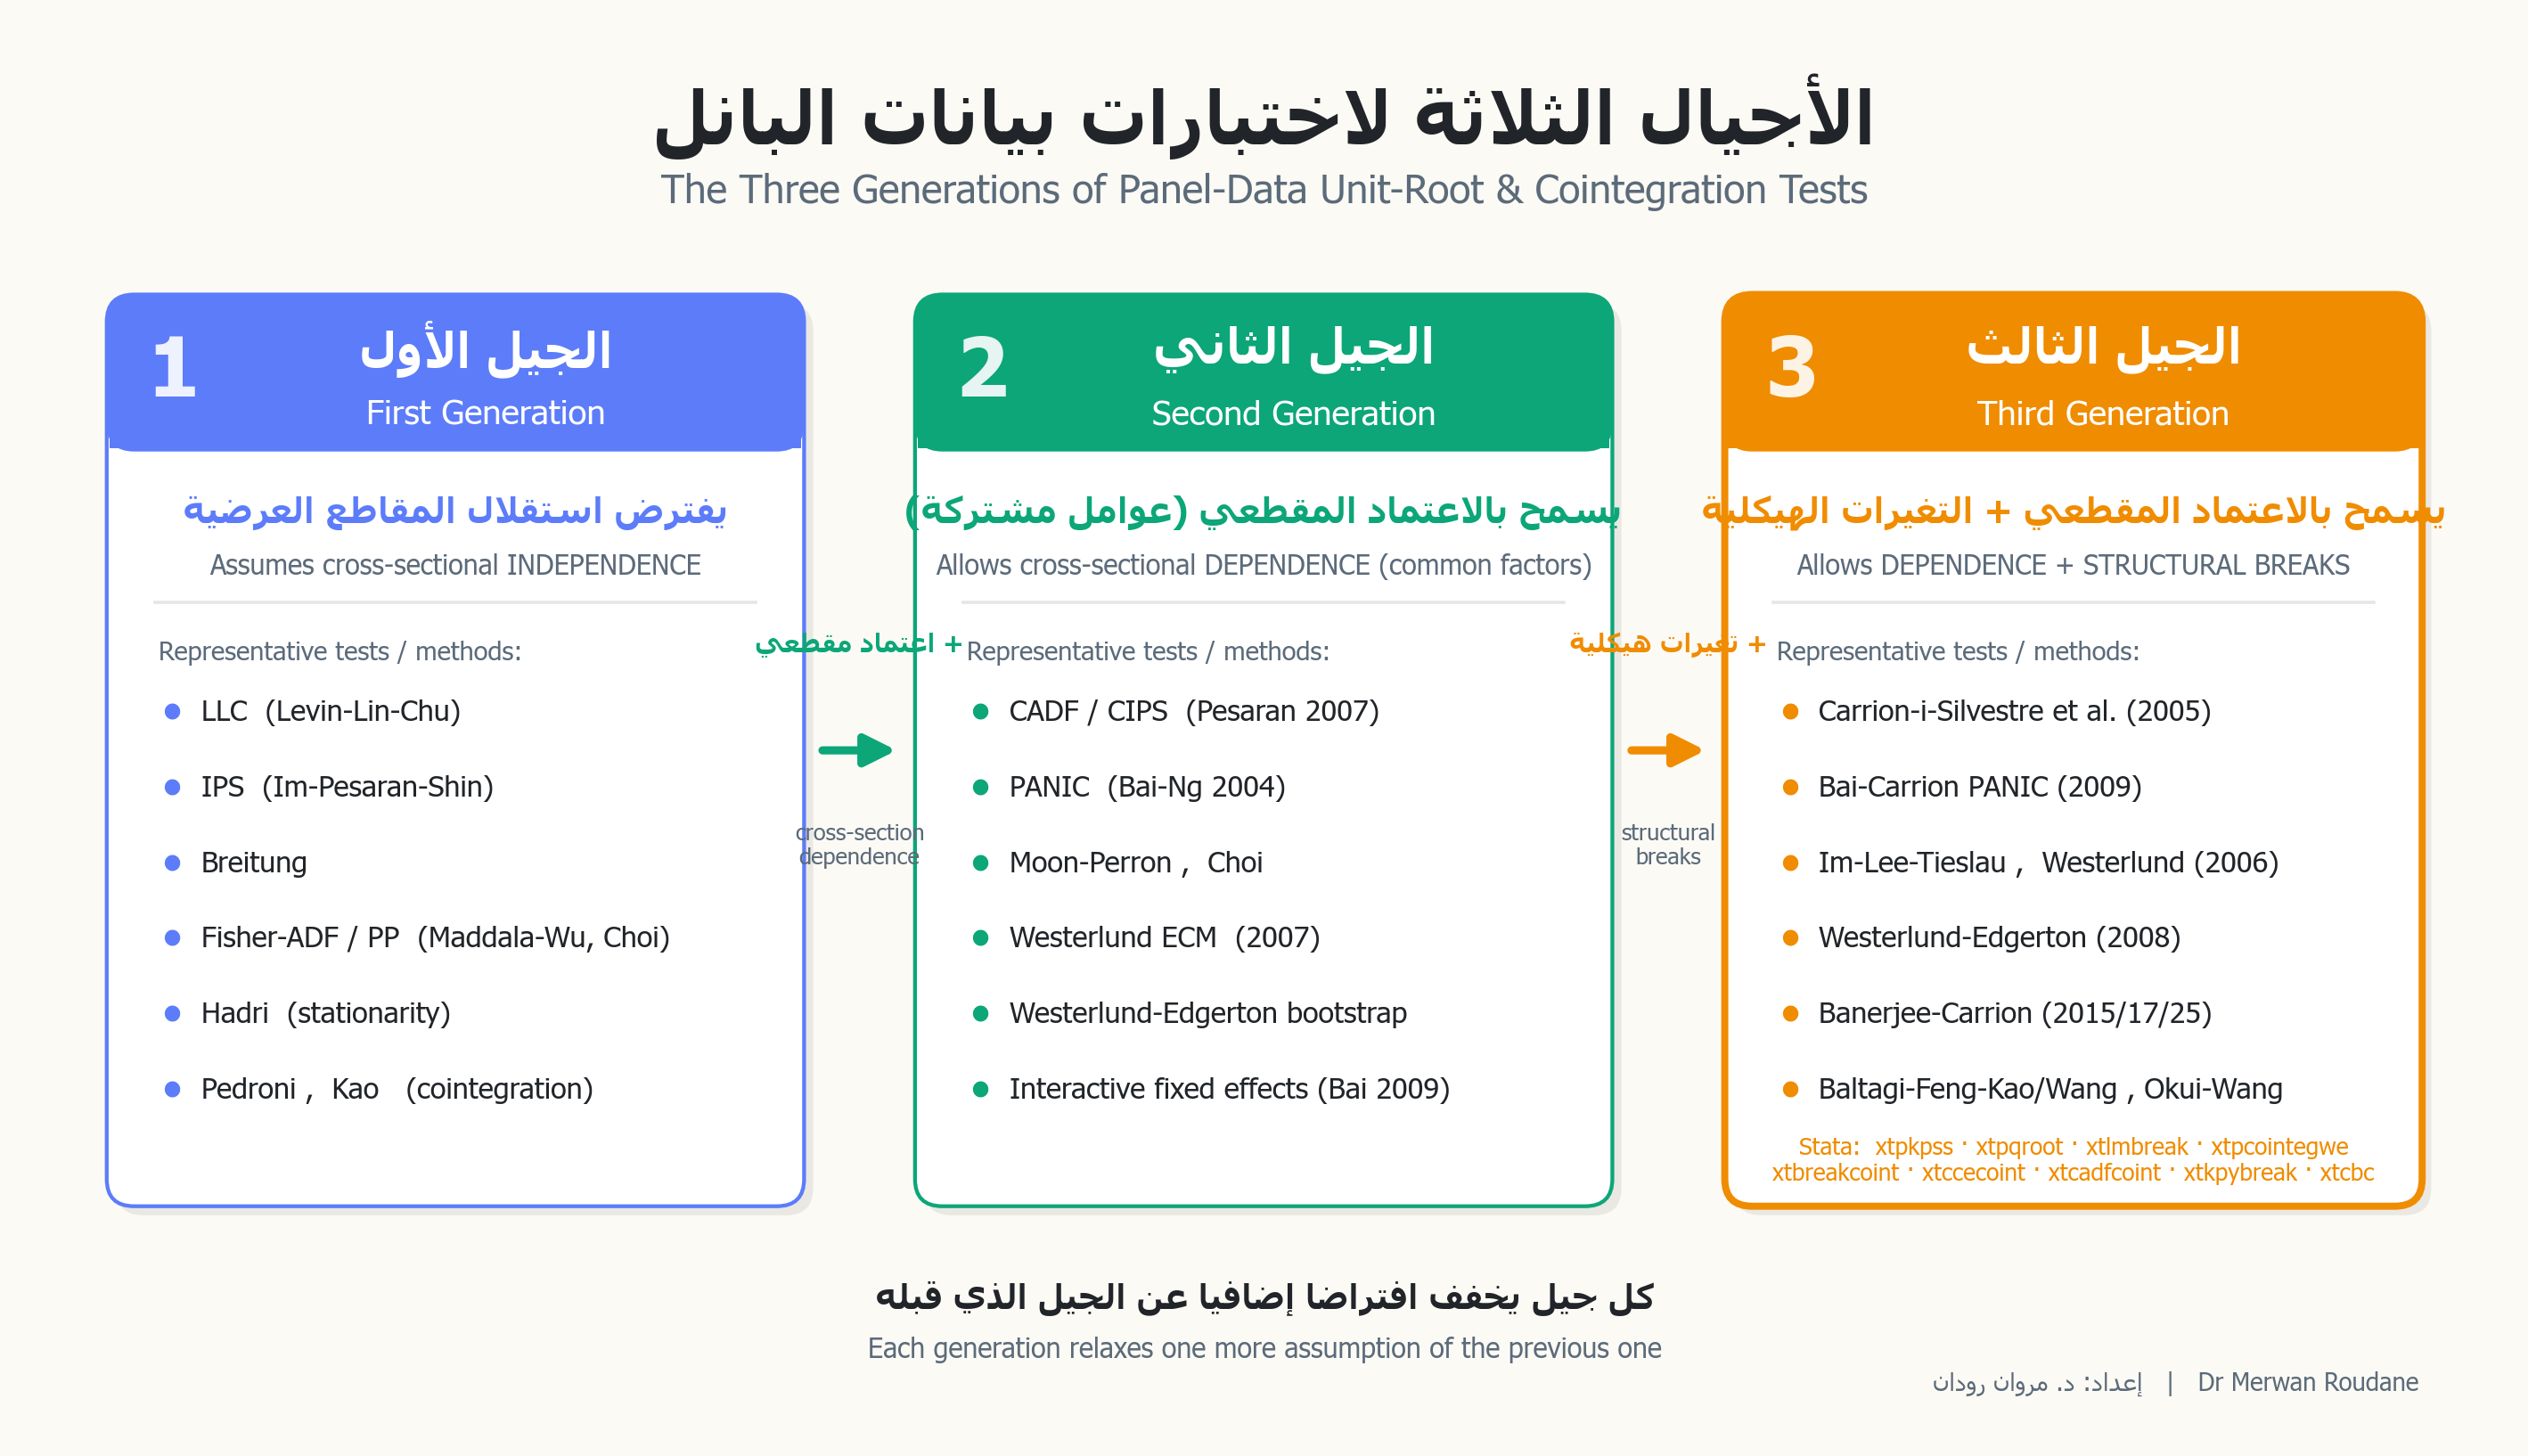
\includegraphics[width=\linewidth]{panel_three_generations.png}\par
\vspace{0.9cm}
{\large\bfseries\color{cgrape} Dr Merwan Roudane\par}
{\color{cgray} Author of the \texttt{xt*} panel structural-break Stata suite (100+ modules)\par}
{\color{cgray}\small ideas.repec.org/f/pro1421 \quad$\cdot$\quad github.com/merwanroudane\par}
\vfill
{\color{cgray}\small Lecture notes: pre-concepts, tests, estimators, regularization, Fourier methods, and software}
\end{titlepage}

\tableofcontents
\newpage

% ======================= NOTATION =======================
\section*{Notation and symbols}
\addcontentsline{toc}{section}{Notation and symbols}
\markboth{Notation and symbols}{}
\renewcommand{\arraystretch}{1.25}
\rowcolors{2}{rowtint}{white}
\begin{center}
\begin{tabular}{@{}>{\color{cblue}\ttfamily}l >{\raggedright\arraybackslash}p{12.4cm}@{}}
\rowcolor{cblue}\color{white}\bfseries Symbol & \color{white}\bfseries Meaning\\
$i,\;t$ & unit index $i=1,\dots,N$; time index $t=1,\dots,T$\\
$N,\;T$ & number of cross-sectional units; number of time periods\\
$y_{it},\;\bx_{it}$ & dependent variable; vector of $K$ regressors for unit $i$ at time $t$\\
$\alpha_i$ & individual (fixed) effect --- unit-specific intercept\\
$\bbeta,\;\bbeta_i(t)$ & slope vector; time-varying / unit-specific slope (breaks live here)\\
$\bff_t,\;\bgamma_i$ & unobserved common factors; unit-specific factor loadings\\
$e_{it},\;\varepsilon_{it}$ & idiosyncratic errors\\
$T_B,\;\lambda=T_B/T$ & break date; break fraction (relative position in the sample)\\
$\omega^2$ & long-run variance (LRV)\\
$\lambda$ (penalty) & regularization tuning parameter (context makes it clear)\\
$\rho_i$ & autoregressive / persistence coefficient of unit $i$\\
$\Delta$ & first-difference operator, $\Delta y_t=y_t-y_{t-1}$\\
\end{tabular}
\end{center}
\rowcolors{1}{}{}
\renewcommand{\arraystretch}{1.0}

% ======================= INTRO =======================
\section{Introduction: what this lecture is about}

Modern applied panel work must survive \emph{three} problems \emph{at the same time}:
\begin{enumerate}[leftmargin=1.5em,itemsep=1pt]
  \item the series may be \hlt{cblue}{non-stationary} (unit roots / stochastic trends);
  \item the units may be \hlt{ccyan}{cross-sectionally dependent} (they share global shocks);
  \item the relationships may contain \hlt{camber}{structural breaks} (they shift at some dates).
\end{enumerate}
Tools that handle all three together are \hlt{cgrape}{third-generation} methods. This lecture builds
them from zero: pre-concepts first, then the anatomy of a break, then cross-sectional dependence,
then the three modern toolkits for modelling breaks (\hlt{cblue}{dummies}, \hlt{cgrape}{Fourier},
\hlt{cteal}{regularization}), and finally the full catalogue of tests and estimators --- with
\textbf{GAGFL}, \textbf{coefficient-by-coefficient (CBC)}, \textbf{Fourier CCEMG} and
\textbf{Fourier panel ARDL} explained in detail, and Stata code for every step.

\begin{begbox}
No prior econometrics beyond a first regression course is assumed. Every symbol is explained the
first time it appears. \hlt{cteal}{Teal boxes} give the plain-English version; \hlt{cgrape}{purple
boxes} are worked examples; \hlt{cred}{red boxes} flag common mistakes; \hlt{camber}{amber boxes}
state the key idea; \hlt{ccyan}{cyan boxes} highlight the central equation.
\end{begbox}

% ======================= PART I =======================
\section{Part I --- Foundations from zero}

\subsection{The panel and its two dimensions}
A \emph{panel} (or \emph{longitudinal}) dataset follows the same $N$ units over $T$ periods, giving
$NT$ observations. The basic linear panel model is
\begin{equation}
y_{it}=\alpha_i+\bx_{it}'\bbeta+u_{it},\qquad i=1,\dots,N;\ t=1,\dots,T,
\end{equation}
where $\alpha_i$ (the \hlt{cblue}{fixed effect}) absorbs all time-invariant, unit-specific
heterogeneity. Two devices remove $\alpha_i$:
\begin{itemize}[leftmargin=1.4em,itemsep=1pt]
 \item \textbf{Within transformation:} subtract each unit's time-mean,
 $\ddot y_{it}=y_{it}-\bar y_{i\cdot}$, killing $\alpha_i$;
 \item \textbf{First differencing:} $\Delta y_{it}=y_{it}-y_{i,t-1}$, also killing $\alpha_i$.
\end{itemize}

\begin{definition}[Two asymptotic regimes --- why they matter]
\begin{itemize}[leftmargin=1.2em,itemsep=1pt]
 \item \hlt{cblue}{Fixed-$T$, large-$N$}: $N\to\infty$, $T$ small (micro panels; many macro panels).
 Break-date and factor consistency then come from having \emph{many units}. Carrion et al.\ (2005),
 Kaddoura (2025), Baltagi--Feng--Kao work here.
 \item \hlt{cblue}{Large-$T$}: $T\to\infty$ (alone or jointly with $N$). Needed for unit-root /
 cointegration limits built on \emph{Brownian motion}. Westerlund (2006), KPY (2011),
 Banerjee--Carrion work here.
\end{itemize}
Using a fixed-$T$ test on a short panel is fine; using a large-$T$ test on $T=8$ is not.
\end{definition}

\subsection{Stationarity, unit roots, and integration}
A series is \hlt{cteal}{stationary} (\Izero) if its mean and variance are constant and its
autocovariances die out. It is \hlt{cred}{integrated of order one} (\Ito) if it must be differenced
once to become \Izero. The canonical \Ito{} process is the \emph{random walk}
\begin{equation}
y_t=y_{t-1}+\varepsilon_t \iff \Delta y_t=\varepsilon_t,\qquad \varepsilon_t\sim(0,\sigma^2),
\end{equation}
for which $\mathrm{Var}(y_t)=t\sigma^2$ \emph{grows without bound} --- shocks are \emph{permanent}.
In an AR(1) $y_t=\rho y_{t-1}+\varepsilon_t$, a \hlt{cred}{unit root} is $\rho=1$; if $|\rho|<1$ the
series is mean-reverting and shocks are transitory.

\begin{begbox}[Difference-stationary vs trend-stationary]
Both an \Ito{} series and a trend-stationary series can drift upward. But the \Ito{} one has a
\emph{stochastic} trend (remove it by \emph{differencing}); the trend-stationary one has a
\emph{deterministic} trend (remove it by \emph{de-trending}). Mixing them up is the root of the
\hlt{cred}{Perron critique} (Section~4.3): an unmodelled break makes a stationary series \emph{look}
like a unit root.
\end{begbox}

\subsubsection{Two families of test: ADF vs KPSS}
\begin{center}
\rowcolors{2}{rowtint}{white}
\begin{tabular}{@{}>{\bfseries}l l l l@{}}
\rowcolor{cteal}\color{white}Family & \color{white}$H_0$ & \color{white}Reject means & \color{white}Panel-with-breaks\\
ADF / DF-type & unit root & stationarity & Im--Lee--Tieslau; CIPS; \cmd{xtpqroot}\\
KPSS / Hadri & stationarity & unit root & Carrion et al.; \cmd{xtpkpss}\\
\end{tabular}
\rowcolors{1}{}{}
\end{center}
The KPSS statistic uses \emph{partial sums} of residuals:
\begin{eqbox}[The KPSS engine (drives xtpkpss)]
\[
\text{KPSS}=\frac{1}{T^2\hat\omega^2}\sum_{t=1}^{T}S_t^2,\qquad S_t=\sum_{s=1}^{t}\hat\varepsilon_s .
\]
\end{eqbox}
Under stationarity $S_t$ stays bounded; under a unit root it wanders and inflates the statistic.

\begin{definition}[Long-run variance (LRV) and how it is estimated]
The LRV is the spectral density at frequency zero,
\[
\omega^2=\gamma(0)+2\sum_{k=1}^{\infty}\gamma(k),\qquad \gamma(k)=\mathrm{Cov}(u_t,u_{t-k}),
\]
estimated by a kernel (HAC) estimator with bandwidth $\ell$:
$\hat\omega^2=\hat\gamma(0)+2\sum_{k=1}^{\ell}w(k/\ell)\hat\gamma(k)$, where $w(\cdot)$ is the
\hlt{ccyan}{Bartlett} or \hlt{ccyan}{Quadratic-Spectral} kernel and $\ell$ the Andrews--Schwarz
bandwidth $\lfloor 4(T/100)^{2/9}\rfloor$. The \hlt{cblue}{homogeneous} version pools one $\omega^2$;
the \hlt{cblue}{heterogeneous} version allows a different $\omega_i^2$ per unit (exactly the
$Z_{\mathrm{hom}}$ vs $Z_{\mathrm{het}}$ split in \cmd{xtpkpss}).
\end{definition}

\subsection{Spurious regression and cointegration}
\begin{exbox}[The spurious-regression trap]
Simulate two \emph{independent} random walks $y_t,x_t$ and regress $y$ on $x$. You will typically get
$R^2>0.7$ and a huge $t$-statistic --- yet there is \emph{no} relationship. The residuals are \Ito{}
(strongly autocorrelated), which is the tell-tale sign. \textbf{Lesson:} never run OLS on \Ito{}
levels without checking cointegration first.
\end{exbox}
Two \Ito{} series are \hlt{cteal}{cointegrated} if a linear combination of them is \Izero:
\begin{equation}
y_{it}=\alpha_i+\bbeta_i'\bx_{it}+e_{it},\qquad \bx_{it}\sim\Ito,\ e_{it}\sim\Izero
\ \Rightarrow\ \text{cointegration.}
\end{equation}
Equivalently there is an \hlt{camber}{error-correction} form with adjustment speed $\phi_i<0$:
\begin{equation}
\Delta y_{it}=\phi_i\big(y_{i,t-1}-\bbeta_i'\bx_{i,t-1}\big)+\text{(short-run terms)}+\varepsilon_{it}.
\end{equation}
A \hlt{camber}{structural break in cointegration} means $\alpha_i$ and/or $\bbeta_i$ shift at some
date --- the equilibrium itself moves.

\subsection{Why ``generations''?}
See the front-page figure. Each generation drops one more convenient assumption:
\hlt{cblue}{1st} assumes independence; \hlt{ccyan}{2nd} allows dependence but no breaks;
\hlt{cgrape}{3rd} allows dependence \emph{and} breaks. The rest of the lecture is the third column.

% ======================= PART II =======================
\section{Part II --- Anatomy of a structural break}

\subsection{Decomposition: where a break lives}
\begin{eqbox}[The master decomposition]
\[
y_{it}=\underbrace{D_{it}}_{\text{deterministics (breaks here)}}
+\underbrace{\bgamma_i'\bff_t}_{\text{common factor = dependence}}
+\underbrace{e_{it}}_{\text{idiosyncratic}} .
\]
\end{eqbox}

\begin{definition}[Structural break]
A change, at one or more dates $T_B$, in the parameters generating the data --- the intercept, the
trend, the slope, or the factor loadings.
\end{definition}

\subsection{Sharp breaks: level, trend, regime}
Let $DU_t=\mathbf 1\{t>T_B\}$ and $DT_t=(t-T_B)^+$. The three Perron-type sharp models are:
\begin{align}
\text{(A) level shift:}\quad & D_{it}=\mu_i+\theta_i\,DU_t,\\
\text{(B) trend break:}\quad & D_{it}=\mu_i+\beta_i t+\delta_i\,DT_t,\\
\text{(C) regime shift:}\quad & D_{it}=\mu_i+\theta_i\,DU_t+\beta_i t+\delta_i\,DT_t.
\end{align}
\begin{exbox}[Reading a level shift]
Suppose GDP growth averages $2\%$ before 2008 and $1\%$ after. Then $\mu_i=2$, $\theta_i=-1$,
$T_B=2008$. A test that ignores $\theta_i\,DU_t$ sees a series that ``fails to revert to $2\%$'' and
wrongly concludes a unit root --- the Perron critique in one line.
\end{exbox}

\subsection{Where the break sits (four possibilities)}
\begin{center}
\rowcolors{2}{rowtint}{white}
\begin{tabular}{@{}>{\bfseries}l p{7.6cm} l@{}}
\rowcolor{camber}\color{white}Break in & \color{white}Meaning & \color{white}Handled by\\
intercept & the mean level shifts & \cmd{xtpkpss}, \cmd{xtpcointegwe}\\
slope $\bbeta(t)$ & the marginal effect of $\bx$ changes & \cmd{xtbreakmodel}, \cmd{xtcbc}\\
cointegrating vector & the long-run equilibrium shifts & \cmd{xtbreakcoint}, \cmd{xtcadfcoint}\\
factor loadings $\bgamma_i(t)$ & sensitivity to the common shock changes & \cmd{xtkpybreak}\\
\end{tabular}
\rowcolors{1}{}{}
\end{center}

\subsection{Common vs heterogeneous breaks (across units)}
\begin{definition}[Common / grouped / heterogeneous]
\hlt{cblue}{Common}: all units break at the same dates,
$\bbeta_i(t)=\bbeta_j$ for $T_{j-1}<t\le T_j$ with the same $T_1,\dots,T_m$ for every $i$.
\hlt{cteal}{Grouped}: units cluster into $G$ latent groups, each group with its own dates.
\hlt{camber}{Heterogeneous}: each unit has its own dates.
\end{definition}
\begin{keyidea}
Fewer distinct break schedules $\Rightarrow$ fewer parameters $\Rightarrow$ more power \emph{if} the
restriction is true. Common (1 schedule) $\subset$ Grouped ($G$ schedules) $\subset$ Heterogeneous
($N$ schedules). GAGFL estimates the grouped case; CCE-break methods assume common breaks; Fourier
CCEMG absorbs heterogeneous-date breaks.
\end{keyidea}

\subsection{Vector vs coefficient-by-coefficient (across coefficients)}
\begin{center}
\rowcolors{2}{rowtint}{white}
\begin{tabular}{@{}>{\bfseries}l p{8.6cm} l@{}}
\rowcolor{cgrape}\color{white}Type & \color{white}Rule & \color{white}Command\\
Vector break & all $K$ coefficients break together at each $T_B$ & \cmd{xtbreakmodel}\\
Coefficient-by-coefficient & each $\beta_k(t)$ breaks on its own schedule & \cmd{xtcbc}\\
\end{tabular}
\rowcolors{1}{}{}
\end{center}
Vector breaks over-split (they break stable coefficients too); CBC avoids this (Section~7.5).

\subsection{Sharp vs smooth breaks}
\begin{definition}[Sharp vs smooth]
\hlt{cred}{Sharp} = step (dummy) at $T_B$. \hlt{cgrape}{Smooth} = gradual transition, modelled by
\begin{align}
\text{logistic STR:}\quad & F(t)=\big[1+\exp(-\gamma(t/T-\tau))\big]^{-1},\\
\text{Fourier:}\quad & d_t=a_0+\textstyle\sum_k\big[a_k\sin\tfrac{2\pi k t}{T}+b_k\cos\tfrac{2\pi k t}{T}\big].
\end{align}
$\gamma$ sets sharpness ($\gamma\to\infty$ is a step), $\tau$ the location; a few Fourier frequencies
$k$ capture unknown, multiple, smooth breaks \emph{with no date to estimate}.
\end{definition}

\subsection{A seven-question checklist}
Answer these and the correct family is essentially pinned down:
\begin{enumerate}[leftmargin=1.5em,itemsep=0pt]
 \item Level, trend, or regime shift? \quad 2. Intercept, slope, cointegrating vector, or loadings?
 \item One or several breaks? \quad 4. Known or estimated dates?
 \item Common, grouped, or heterogeneous across units?
 \item Vector or coefficient-by-coefficient? \quad 7. Sharp or smooth?
\end{enumerate}
Then always add: is there \hlt{ccyan}{cross-sectional dependence} and \hlt{cred}{non-stationarity}?
(In this literature, almost always yes.)

% ======================= PART III =======================
\section{Part III --- Cross-sectional dependence (CSD)}

\subsection{What CSD is and why first-generation tests fail}
\begin{eqbox}[Common-factor error structure]
\[
u_{it}=\bgamma_i'\bff_t+\varepsilon_{it},\qquad
\bff_t=(f_{1t},\dots,f_{rt})'\ \text{unobserved common factors.}
\]
\end{eqbox}
$\bff_t$ is the shared shock (oil, crises, technology); $\bgamma_i$ is unit $i$'s exposure. The
regressors load on the same factors, $\bx_{it}=\Gamma_i'\bff_t+\mathbf v_{it}$, which is exactly what
makes the CCE proxy work.
\begin{warnbox}
Ignore $\bff_t$ and first-generation tests \textbf{over-reject} the unit-root null: the shared shock
induces correlation across units that the ``independent-panel'' variance formula does not account
for, so the pooled statistic is too large. You will ``find'' stationarity or cointegration that is an
artefact of the common shock.
\end{warnbox}

\subsection{Two ways to remove CSD}
\subsubsection{(a) Cross-sectional averages --- CCE (Pesaran, 2006)}
Use $\bar y_t=\frac1N\sum_j y_{jt}$ and $\bar\bx_t=\frac1N\sum_j\bx_{jt}$ as proxies for $\bff_t$ and
partial them out. With $\bar Z=[\bar y,\bar X]$ and $\bar M=I-\bar Z(\bar Z'\bar Z)^{-1}\bar Z'$,
\begin{eqbox}[CCE mean-group / pooled slope]
\[
\hat\bbeta_i=(X_i'\bar M X_i)^{-1}X_i'\bar M y_i,\qquad
\hat\bbeta_{\mathrm{CCEMG}}=\frac1N\sum_{i}\hat\bbeta_i,\qquad
\hat\bbeta_{\mathrm{CCEP}}=\Big(\sum_i X_i'\bar M X_i\Big)^{-1}\sum_i X_i'\bar M y_i.
\]
\end{eqbox}
\hlt{cred}{Remarkable (KPY 2011):} this stays valid even when $\bff_t$ is \Ito. That is the linchpin
behind \cmd{xtkpybreak}.

\subsubsection{(b) Common factors --- PANIC / principal components (Bai--Ng, 2004)}
Estimate the factors explicitly. Since levels mix integration orders, \emph{difference first},
extract factors from differences by PCA, then re-cumulate:
\begin{equation}
\Delta y_{it}=\bgamma_i'\Delta\bff_t+\Delta e_{it}\ \xrightarrow{\text{PCA}}\
\widehat{\bff}_t=\textstyle\sum_{s\le t}\Delta\widehat{\bff}_s,\quad
\hat e_{it}=\sum_{s\le t}\Delta\hat e_{is},
\end{equation}
and test $\widehat{\bff}_t$ and $\hat e_{it}$ separately for unit roots. The number of factors $r$ is
chosen by the Bai--Ng criterion
\begin{equation}
\mathrm{IC}_{p2}(k)=\ln\!\big(V(k,\widehat F^k)\big)+k\Big(\tfrac{N+T}{NT}\Big)\ln\!\big(\min\{N,T\}\big),
\end{equation}
minimised over $k$.
\begin{keyidea}[Averages vs factors, in one line]
\hlt{cblue}{CCE} = don't estimate the factors, subtract their footprint (cross-section averages).
\hlt{cgrape}{PANIC} = estimate the factors by PCA. CCE is simpler; PANIC additionally tells you
\emph{whether} the non-stationarity is common or idiosyncratic.
\end{keyidea}

\subsection{The degree of dependence: classic binary vs modern}
\begin{begbox}[Classic vs modern view]
Classic: ``is there dependence --- yes or no?'' Modern: \emph{how strong}, indexed by the exponent
$\alpha$ in $\sum_i|\gamma_i|=O(N^{\alpha})$:
\begin{itemize}[leftmargin=1.2em,itemsep=0pt]
 \item $\alpha=1$: \hlt{cred}{strong} (a genuine common factor). CCE/PANIC designed for this.
 \item $1/2<\alpha<1$: \hlt{camber}{semi-weak}. Banerjee--Carrion (2017) study CCE here.
 \item $\alpha\le 1/2$: \hlt{cteal}{weak / spatial} (local dependence). Spatial models / robust s.e.
\end{itemize}
\end{begbox}

\subsection{Detecting CSD: the CD test}
\begin{eqbox}[Pesaran CD test]
\[
CD=\sqrt{\frac{2T}{N(N-1)}}\sum_{i<j}\hat\rho_{ij}\ \xrightarrow{d}\ N(0,1),\qquad
\hat\rho_{ij}=\text{pairwise residual correlation.}
\]
\end{eqbox}
Reject $\Rightarrow$ dependence is present $\Rightarrow$ use 2nd/3rd-generation tools. Stata:
\begin{lstlisting}
xtset id year
xtcd2 resid          // Pesaran CD test on residuals (after a regression)
\end{lstlisting}

% ======================= PART IV =======================
\section{Part IV --- Types of tests: classic vs modern}

\subsection{Classic: existence (yes / no)}
Classic tests answer a binary question --- unit root yes/no, cointegration yes/no.
\begin{warnbox}[The null-direction trap]
Half the cointegration tests have $H_0=$ cointegration (residual/LM: Westerlund 2006,
\cmd{xtpcointegboot}) and half $H_0=$ no cointegration (ECM/factor: \cmd{xtpcointegwe},
\cmd{xtbreakcoint}). ``Reject'' means \emph{opposite} things. State the null before the p-value.
\end{warnbox}

\subsection{Confirmatory analysis}
Because unit-root and stationarity tests have low power, best practice is \hlt{cblue}{confirmatory
analysis}: run \emph{both} an ADF-type ($H_0$: unit root) and a KPSS-type ($H_0$: stationarity). If
they agree (one rejects, the other does not), the conclusion is robust; if both reject or neither
rejects, the data are uninformative and you should be cautious.

\subsection{Modern: the degree, not just the fact}
Third-generation tests move from ``exists / doesn't'' to \emph{how much}:
\begin{itemize}[leftmargin=1.4em,itemsep=0pt]
 \item \hlt{cpink}{persistence across quantiles} --- mean-reverting in calm times, persistent in the
 tails (CIPS$(\tau)$; \cmd{xtpqroot});
 \item \hlt{ccyan}{strength of dependence} --- weak / semi-weak / strong;
 \item \hlt{camber}{asymmetric adjustment} --- faster correction on one side (nonlinear ECM;
 \cmd{xtnonlincoint}).
\end{itemize}

% ======================= PART V =======================
\section{Part V --- Three toolkits for modelling breaks}

\begin{center}
\rowcolors{2}{rowtint}{white}
\begin{tabular}{@{}>{\bfseries}p{2.8cm} p{6.2cm} p{5.4cm}@{}}
\rowcolor{cblue}\color{white}Toolkit & \color{white}How it models the break & \color{white}Best when\\
A. Dummies & step dummies at estimated dates (sharp) & discrete events, clear dates\\
B. Fourier & sine/cosine terms for smooth change & gradual / unknown-number breaks\\
C. Regularization & a penalty shrinking tiny changes to zero, keeping real breaks & many candidate
dates, automatic selection\\
\end{tabular}
\rowcolors{1}{}{}
\end{center}
Toolkit A is Section~8 (Bai--Perron, Carrion KPSS, Westerlund). Toolkit B is Section~7 (Fourier).
Toolkit C is Section~6 (regularization). We take C and B first because they are the modern, less
familiar tools.

% ======================= PART VI =======================
\section{Part VI --- Regularization explained, and GAGFL / PLS / CBC}

\subsection{What is regularization? (from zero)}
\begin{begbox}[The overfitting problem]
Give a model as many free parameters as data points and it fits the sample perfectly but predicts
terribly --- it memorised noise. \hlt{cteal}{Regularization} adds a \emph{penalty} for complexity,
trading a little bias for a big drop in variance.
\end{begbox}
The \hlt{cblue}{bias--variance decomposition} of prediction error is
\begin{equation}
\E[(y-\hat y)^2]=\underbrace{(\text{Bias})^2}_{\uparrow\text{ with }\lambda}
+\underbrace{\text{Variance}}_{\downarrow\text{ with }\lambda}+\text{noise},
\end{equation}
so there is an optimal penalty $\lambda^\ast$ that minimises the total. A regularized estimator solves
\begin{eqbox}[Fit + penalty]
\[
\min_{\bbeta}\ \underbrace{\sum_{i,t}(y_{it}-\bx_{it}'\bbeta)^2}_{\text{fidelity}}
\;+\;\lambda\cdot\underbrace{\mathrm{pen}(\bbeta)}_{\text{complexity}} ,\qquad \lambda\ge 0.
\]
\end{eqbox}

\subsubsection{Ridge, lasso, and why lasso hits zero}
\begin{center}
\rowcolors{2}{rowtint}{white}
\begin{tabular}{@{}>{\bfseries}l l p{7.8cm}@{}}
\rowcolor{cteal}\color{white}Penalty & \color{white}Form & \color{white}Effect\\
Ridge ($\ell_2$) & $\lambda\sum_k\beta_k^2$ & shrinks all coefficients, none exactly to zero\\
Lasso ($\ell_1$) & $\lambda\sum_k|\beta_k|$ & shrinks some coefficients \emph{exactly} to zero (selection)\\
Fused lasso & $\lambda\sum_t|\beta_t-\beta_{t-1}|$ & fuses consecutive periods into constant regimes\\
\end{tabular}
\rowcolors{1}{}{}
\end{center}
The lasso hits exactly zero because its constraint region $\sum|\beta_k|\le c$ is a
\emph{diamond} with sharp corners on the axes; the elliptical fit contours touch a corner (a zero
coefficient) with positive probability. The scalar solution is \hlt{camber}{soft-thresholding}:
\begin{equation}
\hat\beta^{\text{lasso}}=\mathrm{sign}(\hat\beta^{\text{OLS}})\,\big(|\hat\beta^{\text{OLS}}|-\lambda\big)^+ .
\end{equation}

\subsubsection{Fused lasso = automatic break detection}
\begin{keyidea}
Penalise $|\beta_t-\beta_{t-1}|$. Most consecutive differences are shrunk to \emph{exactly} zero (the
coefficient is constant across those periods); the few non-zero differences are the \hlt{camber}{break
dates}. So break detection becomes variable selection --- no need to pre-specify the number of breaks.
\end{keyidea}
For a \emph{vector} coefficient we penalise the group norm $\lVert\bbeta_t-\bbeta_{t-1}\rVert$
(\hlt{cblue}{group fused lasso}) and use \hlt{cblue}{adaptive weights} for the oracle property:
\begin{eqbox}[Adaptive group fused lasso (the workhorse)]
\[
\min_{\{\bbeta_t\}}\ \frac1N\sum_{i,t}\big(y_{it}-\bx_{it}'\bbeta_t\big)^2
+\lambda\sum_{t=2}^{T}w_t\,\lVert\bbeta_t-\bbeta_{t-1}\rVert,\qquad
w_t=\lVert\dot\bbeta_t-\dot\bbeta_{t-1}\rVert^{-\kappa}.
\]
\end{eqbox}
$\dot\bbeta_t$ are pilot estimates; $\kappa$ (often $2$) is the adaptive exponent; adaptive weighting
gives the \hlt{cred}{oracle property} (asymptotically finds the true breaks as if known). The penalty
$\lambda$ is picked by a BIC-type information criterion.

\subsubsection{How it is computed: block coordinate descent (BCD)}
The objective is convex but non-smooth. \hlt{cblue}{Block coordinate descent} updates one period's
$\bbeta_t$ at a time, holding the rest fixed, via a soft-thresholding / scalar line-search step; a
full sweep $t=1,\dots,T$ is repeated until the coefficient path stabilises. If the update norm falls
below $\lambda w_{t-1}$, the block is \emph{fused} to the previous period ($\bbeta_t=\bbeta_{t-1}$).

\subsection{PLS / AGFL --- common breaks (Qian \& Su, 2016)}
The adaptive group fused lasso with a \emph{single common} break schedule for all units. All $K$
coefficients break together at dates selected by the fused penalty; $\lambda$ by BIC. Command:
\cmd{xtbreakmodel, method(pls)}.

\subsection{GAGFL --- grouped heterogeneous breaks (Okui \& Wang, 2021)}
\begin{definition}[GAGFL]
\hlt{cblue}{Grouped Adaptive Group Fused Lasso}: units belong to $G$ latent groups; each group has its
own break dates and regime coefficients; membership is unknown and estimated.
\[
y_{it}=\alpha_i+\bx_{it}'\bbeta_{g_i}(t)+\varepsilon_{it},\qquad g_i\in\{1,\dots,G\}.
\]
\end{definition}
The estimator iterates three stages to convergence:
\begin{step}\textbf{GFE initialisation.} Cluster units into $G$ groups (k-means style,
Bonhomme--Manresa) on their time-varying coefficients, using many random starts to avoid local
minima.\end{step}
\begin{step}\textbf{Group-specific AGFL.} Within each group $g$, solve the adaptive group fused lasso
by BCD to detect that group's break dates and regime coefficients.\end{step}
\begin{step}\textbf{Reassignment.} Move each unit to the group whose estimated coefficient path
minimises its residual sum of squares; return to Step~2.\end{step}
$G$ is chosen by BIC over a grid $G=2,3,\dots$. GAGFL nests common breaks ($G=1$) and captures
cluster-specific timing. Command: \cmd{xtbreakmodel, method(gagfl) groups(\#)}.

\subsection{CBC --- coefficient-by-coefficient breaks (Kaddoura, 2025)}
\begin{definition}[CBC / CBCL]
Each coefficient $\beta_k(t)$ has its \emph{own} number of breaks $m_k$ and dates; stable
coefficients are left unbroken.
\end{definition}
Why it matters: the vector-break assumption splits \emph{every} coefficient at the union of all break
dates, even coefficients that never moved --- inflating variance and masking the time-varying effects.
CBC applies the fused penalty \emph{per coefficient}:
\begin{eqbox}[CBC objective and its information criterion]
\begin{align*}
L_\lambda(\bbeta)&=\frac1N\sum_{i}\sum_{t\ge2}\big(\tilde y_{it}-\bar\bx_{it}'\bbeta\big)^2
+\lambda\sum_{t\ge2}\sum_{k=1}^{K} w_{k,t}\,\lvert\beta_{k,t}-\beta_{k,t-1}\rvert,\\
\text{IC}_1(\lambda)&=\hat\sigma^2(\lambda)+\phi\sum_{k}\big[\hat m_k(\lambda)+1\big],\qquad
\phi=c\,\tfrac{\log N}{\sqrt N}.
\end{align*}
\end{eqbox}
Here $\tilde y_{it}=y_{it}-y_{i1}$ eliminates the fixed effect (first-period deviation), and
$w_{k,t}$ are per-coefficient adaptive weights. \textbf{Sub-regime construction:} for coefficient
$k$ in its regime $j$, the other coefficients $\ell\ne k$ may break at \emph{different} dates, so the
estimator intersects regimes, $r^{(k,j)}_{\ell,c}=r_{k,j}\cap(\ell\text{'s }c\text{-th regime})$, and
builds block-diagonal regressor matrices for the post-selection OLS. The option \cmd{csdemean}
cross-section-demeans to absorb interactive fixed effects (Kaddoura--Westerlund 2023).
\begin{exbox}[The headline result]
In Kaddoura's US county-crime data, the \emph{vector}-break estimator finds 2 breaks in \emph{all 16}
coefficients; \textbf{CBC} finds breaks in only \emph{3} controls, leaving the key deterrence
coefficients unbroken. Command: \cmd{xtcbc}.
\end{exbox}

\subsection{Breaks across quantiles (Zhang et al., 2022)}
Quantile regression $+$ adaptive fused lasso, pooled over quantiles, detects breaks that vary by
quantile level (\cmd{xtquantilebreak}):
\begin{equation}
\min\ \sum_{q}\sum_{i,t}\rho_{\tau_q}\!\big(y_{it}-\alpha_i-\bx_{it}'\bbeta_t(\tau_q)\big)
+\lambda_1\sum_i|\alpha_i|+\lambda_2\sum_{t}w_t\big\lVert\bbeta_t-\bbeta_{t-1}\big\rVert,
\end{equation}
where $\rho_\tau(u)=u(\tau-\mathbf 1\{u<0\})$ is the check function.

% ======================= PART VII =======================
\section{Part VII --- Fourier methods in detail}

\subsection{The flexible Fourier form (FFF)}
\begin{eqbox}[Flexible Fourier deterministic term]
\[
d_t=\alpha_0+\alpha_1 t+\sum_{k=1}^{n}\Big[a_k\sin\!\Big(\tfrac{2\pi k t}{T}\Big)
+b_k\cos\!\Big(\tfrac{2\pi k t}{T}\Big)\Big].
\]
\end{eqbox}
\hlt{cgrape}{Gallant's theorem} (1981): a few low-frequency sine/cosine terms approximate \emph{any}
smooth, bounded deviation, including several gradual breaks. Often a single frequency $n=1$ suffices
(Enders--Lee); the frequency is selected by minimising the SSR, and its significance is checked by an
$F$-test on $(a_k,b_k)$. The \hlt{camber}{fractional frequency} version (Olayeni et al., 2021)
searches non-integer $k\in[0.1,5]$ for a sharper fit --- the FFFFF panel cointegration test.

\subsection{Fourier CCEMG (Guliyev, 2026)}
\begin{keyidea}
When breaks occur at \emph{different dates across units}, dummies explode in number. Fourier CCEMG
augments the CCE regression with \emph{unit-specific} Fourier terms: the cross-section averages filter
the common factor while the Fourier terms \emph{absorb the heterogeneously-timed breaks}.
\end{keyidea}
\begin{eqbox}[Fourier CCEMG unit regression]
\[
y_{it}=\bbeta_i'\bx_{it}
+\underbrace{c_{0i}+c_{1i}\sin\tfrac{2\pi t}{T}+c_{2i}\cos\tfrac{2\pi t}{T}}_{\text{unit-specific smooth breaks}}
+\underbrace{\bdelta_i'\bar{\mathbf z}_t}_{\text{CCE factor proxy}}+\varepsilon_{it},\qquad
\hat\bbeta_{\text{F-CCEMG}}=\frac1N\sum_i\hat\bbeta_i .
\]
\end{eqbox}
with $\bar{\mathbf z}_t=[\bar y_t,\bar\bx_t]$. In Monte Carlo it attains the lowest RMSE across
weak/moderate/strong dependence with near-nominal coverage. (A sister estimator, \hlt{ccyan}{F-SURMG},
augments a seemingly-unrelated system with Fourier terms.)

\subsection{Fourier panel ARDL / CS-ARDL}
The \hlt{cblue}{ARDL} model handles regressors of mixed order (\Izero{} and \Ito) and delivers
long-run and short-run coefficients in one step. The Fourier-augmented panel ARDL lets the long-run
relationship shift \emph{smoothly}; the cross-sectionally augmented (CS-ARDL) version adds
cross-section averages for dependence:
\begin{eqbox}[Fourier CS-ARDL (error-correction form)]
\[
\Delta y_{it}=\phi_i\big(y_{i,t-1}-\btheta_i'\bx_{i,t-1}\big)
+\sum_{j}\bpsi_{ij}'\Delta\bx_{i,t-j}
+\underbrace{\lambda_{1i}\sin\tfrac{2\pi t}{T}+\lambda_{2i}\cos\tfrac{2\pi t}{T}}_{\text{smooth break}}
+\underbrace{\bxi_i'\bar{\mathbf z}_t}_{\text{CS augmentation}}+\varepsilon_{it}.
\]
\end{eqbox}
$\phi_i<0$ is the \hlt{camber}{error-correction (adjustment) speed}; $\btheta_i$ the long-run
coefficients. Averaging the $\hat\btheta_i,\hat\phi_i$ across units gives the \hlt{cblue}{Mean-Group}
estimator; restricting the long-run $\btheta_i=\btheta$ gives the \hlt{cblue}{Pooled Mean Group (PMG)}.
Command: \cmd{xtpfardl}.

% ======================= PART VIII =======================
\section{Part VIII --- The third-generation tests, catalogued}

\subsection{Panel unit-root / stationarity with breaks}
\subsubsection{Panel KPSS with multiple breaks --- Carrion et al.\ (2005) --- \cmd{xtpkpss}}
Each unit's regression allows its own level/trend breaks; the panel averages and standardises:
\begin{eqbox}[Standardised panel KPSS]
\[
Z(\lambda)=\frac{\sqrt N\big(\overline{LM}-\bar\xi\big)}{\sqrt{\bar\varsigma^2}}\ \xrightarrow{d}\ N(0,1),
\qquad \overline{LM}=\frac1N\sum_i LM_i(\lambda_i).
\]
\end{eqbox}
$\bar\xi,\bar\varsigma^2$ are the mean/variance of the individual limit (they depend on the
deterministic model and the break fractions). $H_0$: stationarity; \hlt{cred}{right-tail} rejection.
Homogeneous ($Z_{\mathrm{hom}}$) and heterogeneous ($Z_{\mathrm{het}}$) LRV; dates by Bai--Perron,
number by LWZ, CSD by bootstrap.

\subsubsection{PANIC with breaks --- Bai \& Carrion (2009)}
Add breaks to $D_{it}$, then run PANIC: test the common factors (MQ tests for the number of stochastic
trends) and the pooled idiosyncratic component ($\hat P_e$) separately for unit roots.

\subsubsection{Im--Lee--Tieslau panel LM (2005)}
A score (LM) unit-root test with the break \emph{under the null}, so the statistic is
\hlt{cblue}{invariant} to the break size and location --- estimated dates do not distort its
$N(0,1)$ limit.

\subsubsection{Quantile CIPS and tFR --- \cmd{xtpqroot}}
\hlt{cpink}{CIPS$(\tau)$}: a unit-root test at each quantile (asymmetric persistence).
\hlt{cgrape}{tFR}: smooth (fractional Fourier) $+$ sharp (LST) breaks together, CSD via sieve
bootstrap.
\[
Q_{\Delta y_{it}}(\tau\mid\mathcal F_{t-1})=a_i(\tau)+\rho_i(\tau)y_{i,t-1}+d_i(\tau)\bar y_{t-1}+\cdots,
\qquad H_0:\rho_i(\tau)=1\ \forall i,\tau.
\]

\subsection{Panel cointegration with breaks}
\begin{center}
\rowcolors{2}{rowtint}{white}
\begin{tabular}{@{}>{\bfseries}l >{\ttfamily}l l l@{}}
\rowcolor{cblue}\color{white}Test & \color{white}Command & \color{white}$H_0$ & \color{white}CSD via\\
Westerlund (2006) LM & xtlmbreak & cointegration & bootstrap\\
Westerlund--Edgerton (2008) & xtpcointegwe & no cointegration & common factors\\
Westerlund--Edgerton (2007) & xtpcointegboot & cointegration & sieve bootstrap\\
Banerjee--Carrion (2015) & xtbreakcoint & no cointegration & factors\\
Banerjee--Carrion (2017) & xtccecoint & no cointegration & CCE\\
Banerjee--Carrion (2025) & xtcadfcoint & no cointegration & CCE + factors\\
Nonlinear ECM (2017) & xtnonlincoint & no cointegration & sieve bootstrap\\
\end{tabular}
\rowcolors{1}{}{}
\end{center}
\textbf{Westerlund (2006)} is an LM ($H_0$: cointegration) allowing multiple level/trend breaks at
possibly different dates per unit. \textbf{Westerlund--Edgerton} give a factor-based (2008,
$PD_\tau,PD_\phi$) and a bootstrap ($LM^+$ from FM-OLS, 2007) version. The
\textbf{Banerjee--Carrion trilogy} progressively unifies breaks and dependence; the 2025 test allows
breaks in the deterministic component, the cointegrating vector, \emph{and} the factor loadings
simultaneously. \textbf{Nonlinear ECM} adds asymmetric (regime-dependent) adjustment.

\subsection{CCE with I(1) factors and breaks --- \cmd{xtkpybreak}}
The most fully third-generation \emph{estimator}: CCE robust to \Ito{} factors (KPY 2011) \emph{plus}
multiple breaks in slopes $K_0$ \emph{and} factor loadings $K_1$, estimated jointly by the
dynamic-programming Bai--Perron algorithm (Baltagi--Feng--Wang 2025):
\begin{eqbox}[Nonstationary panel with breaks in slopes and loadings]
\[
y_{it}=\bx_{it}'\bbeta_i(K_0)+\bgamma_i(K_1)'\bff_t+\varepsilon_{it},\qquad \bff_t=\bff_{t-1}+\bphi_t\ (\text{\Ito}).
\]
\end{eqbox}
Empirical example: a common \hlt{camber}{1992 break} in international R\&D spillovers, attributed to
early-1990s globalisation.

\subsection{Estimating and dating breaks: the shared machinery}
\subsubsection{Single break by SSR grid search}
\begin{equation}
\hat T_B=\arg\min_{T_B\in[\varepsilon T,(1-\varepsilon)T]}\ \mathrm{SSR}(T_B),
\end{equation}
with \hlt{cblue}{trimming} $\varepsilon\in[0.10,0.15]$ keeping candidates away from the endpoints.

\subsubsection{Multiple breaks}
By \hlt{cblue}{dynamic programming} (Bai--Perron 2003, global optimum in $O(T^2)$) or
\hlt{cblue}{sequential} detection. The number of breaks is chosen by a sequential
$\sup F(\ell+1\mid\ell)$ test or an information criterion (BIC, LWZ).

\subsubsection{Why the estimated date behaves as if known}
The break fraction is \hlt{cred}{super-consistent}: $T(\hat\lambda-\lambda_0)=O_p(1)$, faster than
$\sqrt T$, so downstream slopes and statistics have the same limit as if $T_B$ were known.

\subsubsection{Pooling to a standard normal}
\begin{equation}
Z=\frac{\sqrt N\big(\overline S-\mu\big)}{\sqrt{\varsigma^2}}\ \xrightarrow{d}\ N(0,1),\qquad
\overline S=\frac1N\sum_i S_i,
\end{equation}
where $(\mu,\varsigma^2)$ are the mean/variance of the individual limit --- \emph{they depend on the
deterministic model and break count}, which is why every paper tabulates a different pair, and why you
must declare the correct \cmd{model()} when you run the command.

% ======================= PART IX =======================
\section{Part IX --- Practical workflow and Stata code}

A defensible ordering for an empirical panel study (all commands from the \cmd{xt*} suite):
\begin{enumerate}[leftmargin=1.5em,itemsep=1pt]
 \item Test for CSD (Pesaran CD). \quad 2. Test and date the breaks.
 \item Unit-root / stationarity, break- and CSD-robust.
 \item Number of common factors. \quad 5. Cointegration with breaks.
 \item Estimate the break-dated coefficients. \quad 7. Interpret the long-run relation.
\end{enumerate}

\begin{lstlisting}
* ---- real data: Grunfeld investment panel (10 firms, 20 years) ----
webuse grunfeld, clear
xtset company year

* 1) cross-sectional dependence
xtcd2 invest                                   // Pesaran CD test

* 3) unit-root / stationarity WITH breaks + CSD
xtpkpss invest, model(constbreak) maxbreaks(2) graph   // H0: stationary
xtpqroot invest, quantile(0.25 0.5 0.75) cdtest        // quantile unit root
xtpqroot invest, fourier model(intercept) bootreps(299)// smooth+sharp breaks

* 5) cointegration WITH breaks + factors
xtpcointegwe   invest mvalue, model(regimeshift) maxfactors(2) graph
xtbreakcoint   invest mvalue kstock, model(levelshift) maxlag(1)
xtcadfcoint    invest mvalue, model(3) breaks(1) nfactors(1) simulate(500)

* 6) estimate the break-dated coefficients
xtbreakmodel invest mvalue, method(pls)                // common vector breaks
xtcbc        invest mvalue kstock, graph               // coefficient-by-coefficient
xtkpybreak   break invest mvalue kstock, nbreaks(1) breakplot   // CCE + I(1) + breaks
\end{lstlisting}

\begin{begbox}[The one sentence to remember]
A third-generation method $=$ \hlt{ccyan}{remove the common factors} (CCE averages or PANIC principal
components) $+$ \hlt{camber}{let the deterministic / coefficient part break} (dummies, Fourier, or a
fused lasso) $+$ \hlt{cblue}{use critical values that know the deterministic model}. Everything else
is which piece each author emphasises.
\end{begbox}

% ======================= PART X: detailed tests =======================
\section{Part X --- Each cointegration test in detail}

\subsection{Westerlund (2006) --- LM test with multiple breaks (\cmd{xtlmbreak})}
An \hlt{cblue}{LM} test whose null is \emph{cointegration}. The cointegrating regression carries
$m_i$ breaks in level and trend, at possibly different dates per unit:
\[
y_{it}=\alpha_i+\textstyle\sum_k\theta_{ik}DU_{ikt}+\beta_i t+\sum_k\delta_{ik}DT_{ikt}+\gamma_i'\bx_{it}+z_{it},
\quad z_{it}=\textstyle\sum_{s\le t}u_{is}.
\]
The individual LM statistic is $LM_i=T^{-2}\sum_t S_{it}^2/\hat\omega_i^2$ (partial sums of the
residuals); the panel statistic $Z(M)=\sqrt N(\overline{LM}-\bar\mu)/\bar\sigma\to N(0,1)$.
\hlt{cred}{Right-tail} rejection $\Rightarrow$ no cointegration. Dates by SSR minimisation, CSD by
bootstrap. \emph{Use it} when you believe in the equilibrium and want to test whether a break
destroys it.

\subsection{Westerlund--Edgerton --- factor and bootstrap versions}
\subsubsection{2008, factor-based (\cmd{xtpcointegwe})}
Individual ADF regressions on the residuals, augmented with break dummies; CSD via a common-factor
structure (PCA, number of factors by Bai--Ng ICp1). Two statistics $PD_\tau$ (t-ratio based) and
$PD_\phi$ (coefficient based), both $\to N(0,1)$. $H_0$: no cointegration; \hlt{cred}{left-tail}
rejection. Models: \cmd{nobreak} / \cmd{levelshift} / \cmd{regimeshift}.
\subsubsection{2007, bootstrap (\cmd{xtpcointegboot})}
The McCoskey--Kao $LM^+$ statistic from \hlt{cblue}{FM-OLS} residuals (which correct endogeneity and
serial correlation). Because asymptotic critical values are poorly sized under CSD, a
\hlt{cblue}{sieve bootstrap} (fit a VAR to the differences, resample innovations) supplies the
critical values. $H_0$: cointegration; right-tail rejection.

\subsection{The Banerjee--Carrion trilogy}
\begin{center}
\rowcolors{2}{rowtint}{white}
\begin{tabular}{@{}>{\bfseries}l p{9.2cm} >{\ttfamily}l@{}}
\rowcolor{cteal}\color{white}Paper & \color{white}What it adds & \color{white}Command\\
2015 (JAE) & cointegration test valid under breaks and CSD (factors) & xtbreakcoint\\
2017 (JTSA) & CCE-based test; consistent long-run parameter under weak/semi-weak/strong dependence & xtccecoint\\
2025 (JBES) & breaks in the deterministic part, the cointegrating vector, AND the factor loadings & xtcadfcoint\\
\end{tabular}
\rowcolors{1}{}{}
\end{center}
The 2025 model (most general) is
\[
y_{it}=D_{it}(\text{breaks})+\theta_i'\bx_{it}(\text{breaks})+\gamma_i(\text{breaks})'\bff_t+e_{it},
\qquad H_0:\,e_{it}\sim\Ito\ (\text{no coint.}).
\]
A defactored CADF-type statistic on the residuals; cross-section averages remove $\bff_t$; break
dates by SSR. \hlt{cred}{Left-tail} rejection $\Rightarrow$ cointegration.

\subsection{Nonlinear ECM cointegration (\cmd{xtnonlincoint})}
The first \hlt{cgrape}{nonlinear} panel cointegration test: adjustment toward equilibrium is
\emph{asymmetric}, modelled by a logistic transition so that the correction speed differs above vs
below the equilibrium; a modified Wald statistic tests the ECM term; CSD via sieve bootstrap:
\[
\Delta y_{it}=\phi_i\,\big[1+\exp(-\gamma_i(e_{i,t-1}-c_i))\big]^{-1} e_{i,t-1}+\text{(short-run)}+\varepsilon_{it},
\qquad H_0:\phi_i=0\ \forall i.
\]

% ======================= PART XI: empirical application =======================
\section{Part XI --- A worked empirical application (narrative)}

Suppose we study the \hlt{cblue}{energy--growth} relationship for $N=20$ countries over
$T=40$ years, with $y=$ log GDP per capita and $x=$ log energy use per capita. Here is the full
third-generation workflow, with how to \emph{read} each step.

\begin{exbox}[Step 1 --- cross-sectional dependence]
Run \cmd{xtcd2}. Suppose $CD=18.4$ ($p<0.001$). \textbf{Read:} strong dependence --- global shocks
(oil prices, crises) hit all countries. First-generation tests are now invalid; we must use CCE /
factor / bootstrap methods.
\end{exbox}
\begin{exbox}[Step 2 --- date the breaks]
Run \cmd{xtgets ... , fesis}. Suppose it flags breaks clustered around 1979 and 2008. \textbf{Read:}
candidate regime changes (oil shock; global financial crisis) --- we will let the tests estimate these
rather than impose them.
\end{exbox}
\begin{exbox}[Step 3 --- unit root with breaks]
Run \cmd{xtpkpss y, model(trendbreak) maxbreaks(2)}. Suppose $Z_{\mathrm{het}}=4.1$ ($p<0.01$).
\textbf{Read:} reject stationarity $\Rightarrow$ $y$ is \Ito{} even after allowing breaks. Repeat for
$x$: also \Ito. Both series are integrated, so a \emph{levels} regression risks being spurious ---
we need cointegration.
\end{exbox}
\begin{exbox}[Step 4 --- cointegration with breaks]
Run \cmd{xtpcointegwe y x, model(regimeshift) maxfactors(2)}. Suppose $PD_\tau=-3.7$ ($p<0.01$).
\textbf{Read:} reject $H_0$ of no cointegration $\Rightarrow$ a long-run energy--growth equilibrium
exists, and it \emph{shifts} at the estimated date. The relationship is real, not spurious.
\end{exbox}
\begin{exbox}[Step 5 --- estimate the break-dated relationship]
Run \cmd{xtkpybreak break y x, nbreaks(1)}. Suppose the long-run elasticity is $0.65$ before the break
and $0.42$ after. \textbf{Read:} energy became \emph{less} tightly linked to growth after the break
(efficiency gains / structural change toward services). Match the estimated date to the real event.
\end{exbox}
\begin{warnbox}[Interpretation discipline]
Always report: (i) the \emph{null} of each test, (ii) the \emph{estimated break dates with a
confidence interval}, and (iii) the \emph{economic event} you attribute each break to. A break with
no story is a red flag for a spurious artefact.
\end{warnbox}

% ======================= FAQ =======================
\section{Beginner FAQ}
\begin{description}[leftmargin=0pt,itemsep=3pt]
\item[\color{cblue}Q. Do I difference before or after removing the factors?]
For PANIC, \emph{difference first}, then extract factors, then re-cumulate. For CCE you do not
difference --- you add the cross-section averages to the levels regression.
\item[\color{cblue}Q. My panel is unbalanced. Can I still use these?]
Most break commands need a \emph{balanced} panel. Balance it first (\cmd{tsfill}, imputation) or use a
missing-value-robust unit-root test as a pre-step.
\item[\color{cblue}Q. How many breaks should I allow?]
Set a sensible \cmd{maxbreaks()} (2--3 for short $T$) and let the information criterion (LWZ/BIC)
choose. Too many candidate breaks on a short $T$ over-fits.
\item[\color{cblue}Q. Dummy, Fourier, or regularization?]
Dummies for \emph{discrete, known-ish} events; Fourier for \emph{gradual / unknown-number} breaks;
regularization when you want the method to \emph{select} the breaks automatically among many candidates.
\item[\color{cblue}Q. Vector break or CBC?]
If you suspect only \emph{some} coefficients move, use CBC (\cmd{xtcbc}); it avoids splitting the
stable ones and keeps their standard errors small.
\item[\color{cblue}Q. What does ``super-consistency'' buy me?]
It means the estimated break date converges so fast that the downstream slope estimates behave
\emph{as if the date were known} --- so you can plug in $\hat T_B$ without an extra penalty.
\end{description}

% ======================= EXERCISES =======================
\section{Exercises}
\begin{enumerate}[leftmargin=1.6em,itemsep=3pt]
 \item \textbf{Concept.} Explain, in one sentence each, the difference between (a) common vs
 heterogeneous breaks, (b) vector vs coefficient-by-coefficient breaks, (c) sharp vs smooth breaks.
 \item \textbf{Null direction.} For each of \cmd{xtpkpss}, \cmd{xtpcointegwe}, \cmd{xtpcointegboot},
 state $H_0$ and what a rejection implies.
 \item \textbf{Regularization.} Starting from the fused-lasso penalty $\lambda\sum_t|\beta_t-\beta_{t-1}|$,
 explain why increasing $\lambda$ reduces the number of detected breaks. What selects $\lambda$?
 \item \textbf{CCE vs PANIC.} Give one situation where you would prefer CCE and one where you would
 prefer PANIC, and justify.
 \item \textbf{Fourier.} Why can a single Fourier frequency approximate several gradual breaks, and why
 is that impossible with a single dummy?
 \item \textbf{Applied (Stata).} On \cmd{webuse grunfeld}, run \cmd{xtcbc invest mvalue kstock, graph}.
 Which coefficients break and which stay constant? Compare with \cmd{xtbreakmodel ..., method(pls)}
 and explain the difference in the number of breaks.
 \item \textbf{Workflow.} Write the seven-step workflow for a panel where the CD test rejects and a
 break is suspected in the long-run slope. Name a command for each step.
\end{enumerate}

% ======================= CHEAT SHEET =======================
\section{One-page cheat-sheet}
\begin{center}
\rowcolors{2}{rowtint}{white}
\begin{tabular}{@{}>{\bfseries}p{3.5cm} p{5.0cm} >{\ttfamily}p{4.6cm}@{}}
\rowcolor{cgrape}\color{white}Question & \color{white}Method & \color{white}Command\\
Is there dependence? & Pesaran CD & xtcd2\\
Detect / date breaks & indicator saturation & xtgets\\
Unit root with breaks? & panel KPSS / quantile CIPS / tFR & xtpkpss, xtpqroot\\
Cointegration with breaks? & Westerlund; Banerjee--Carrion & xtlmbreak, xtpcointegwe, xtbreakcoint, xtccecoint, xtcadfcoint\\
Bootstrap cointegration & FM-OLS $LM^+$ & xtpcointegboot\\
Nonlinear / asymmetric ECM & logistic transition & xtnonlincoint\\
Estimate breaks (common) & Qian--Su / BFK / SaRa & xtbreakmodel\\
Estimate breaks (grouped) & Okui--Wang GAGFL & xtbreakmodel, method(gagfl)\\
Estimate breaks (per-coef) & Kaddoura CBC & xtcbc\\
CCE + I(1) factors + breaks & KPY / Baltagi--Feng--Wang & xtkpybreak\\
Breaks across quantiles & shrinkage QR & xtquantilebreak\\
Endogenous regressor + break & Baltagi--Feng--Kao & xtbfkbreak\\
Dynamic panel, breaks + CSD & robust dynamic estimators & xtdynestimb\\
Panel VAR + cointegration + breaks & panel VECM & xtpvarcoint\\
\end{tabular}
\rowcolors{1}{}{}
\end{center}

% ======================= REFERENCES =======================
\section*{Key references}
\addcontentsline{toc}{section}{Key references}
\markboth{Key references}{}
\small
\begin{itemize}[leftmargin=1.2em,itemsep=1pt]
 \item Bai, J.\ \& Ng, S.\ (2002, 2004). Determining the number of factors; A PANIC attack on unit
 roots and cointegration. \emph{Econometrica} 70(1); 72(4).
 \item Bai, J.\ \& Carrion-i-Silvestre, J.L.\ (2009). Structural changes, common stochastic trends,
 and unit roots in panel data. \emph{Review of Economic Studies} 76(2).
 \item Bai, J.\ \& Perron, P.\ (1998, 2003). Estimating and testing linear models with multiple
 structural changes. \emph{Econometrica} 66(1); \emph{JAE} 18(1).
 \item Baltagi, B.H., Feng, Q.\ \& Kao, C.\ (2016, 2019). Estimation of heterogeneous panels with
 structural breaks. \emph{Journal of Econometrics} 191(1).
 \item Baltagi, B.H., Feng, Q.\ \& Wang, W.\ (2025). Nonstationary heterogeneous panels with multiple
 structural changes. \emph{Econometric Reviews}.
 \item Banerjee, A.\ \& Carrion-i-Silvestre, J.L.\ (2015, 2017, 2025). Panel cointegration with breaks
 and cross-section dependence. \emph{JAE; JTSA; JBES}.
 \item Bonhomme, S.\ \& Manresa, E.\ (2015). Grouped patterns of heterogeneity in panel data.
 \emph{Econometrica} 83(3).
 \item Carrion-i-Silvestre, J.L., del Barrio-Castro, T.\ \& L\'opez-Bazo, E.\ (2005). Breaking the
 panels. \emph{Econometrics Journal} 8(2).
 \item Corakci, A.\ \& Omay, T.\ (2023). Panel unit root test with smooth and sharp breaks.
 \emph{Renewable Energy} 205.
 \item Enders, W.\ \& Lee, J.\ (2012). The flexible Fourier form and unit-root tests.
 \emph{Economics Letters} 117(1).
 \item Kaddoura, Y.\ (2025). Estimating coefficient-by-coefficient breaks in panel data models.
 \emph{Journal of Econometrics} 249.
 \item Kaddoura, Y.\ \& Westerlund, J.\ (2023). Panel models with random interactive effects and
 multiple breaks when $T$ is fixed. \emph{JBES} 41(3).
 \item Kapetanios, G., Pesaran, M.H.\ \& Yamagata, T.\ (2011). Panels with non-stationary multifactor
 error structures. \emph{Journal of Econometrics} 160(2).
 \item Okui, R.\ \& Wang, W.\ (2021). Heterogeneous structural breaks in panel data models.
 \emph{Journal of Econometrics} 220(2).
 \item Olayeni, R.O., Tiwari, A.K.\ \& Wohar, M.E.\ (2021). Fractional frequency flexible Fourier form
 for panel cointegration. \emph{Applied Economics Letters} 28(6).
 \item Pesaran, M.H.\ (2006, 2007). CCE estimation; a simple panel unit-root test.
 \emph{Econometrica; JAE}.
 \item Qian, J.\ \& Su, L.\ (2016). Shrinkage estimation of common breaks via adaptive group fused
 lasso. \emph{Journal of Econometrics} 191(1).
 \item Westerlund, J.\ (2006, 2007); Westerlund, J.\ \& Edgerton, D.L.\ (2007, 2008). Panel
 cointegration with structural breaks. \emph{OBES; Economics Letters}.
 \item Zhang, L., Zhu, Z., Feng, X.\ \& He, Y.\ (2022). Shrinkage quantile regression for panel data
 with multiple structural breaks. \emph{Canadian Journal of Statistics} 50(3).
\end{itemize}

\vfill
\begin{center}\small\color{cgray}
Lecture notes prepared by \textbf{\color{cgrape}Dr Merwan Roudane} --- author of the \texttt{xt*}
panel structural-break Stata suite (ideas.repec.org/f/pro1421 $\cdot$ github.com/merwanroudane).
\end{center}

\end{document}
